% DIV Grösser -> Mehr Text pro Seite
% Bindekorrektur BCOR
% A5
%\usepackage[a5paper,BCOR12mm]{typearea}

\usepackage{kpfonts}
\usepackage{ucs}

% Load symbols like «»
\usepackage[T1]{fontenc} % Load amsmath before this! http://en.wikibooks.org/wiki/LaTeX/Internationalization#Cyrillic_script
% Then load additional utf8 symbols + encoding
\usepackage[utf8x]{inputenc}
\usepackage[russian,ngerman]{babel}

\usepackage{DejaVuSerif}
\newcommand{\ru}[1]{\usefont{T1}{DejaVuSerif-TLF}{m}{n} {\selectlanguage{russian} #1 \selectlanguage{ngerman} \fontfamily{cmr}\selectfont}}
\renewcommand{\rmdefault}{cmr}

\usepackage{xcolor}
\usepackage{fontenc}
\usepackage{graphicx}

\usepackage[dvips,pdftex,pdfusetitle]{hyperref}

% Math environments
\usepackage{amsmath}
\usepackage{amsfonts}

\usepackage{calc}

% For top/mid/bottomrule
\usepackage{booktabs}

\usepackage{xtab}
\usepackage{longtable}
\usepackage{tabu}
\usepackage{colortbl}

\usepackage{rotating}
\usepackage{varwidth}

% Bash
% Table LibO -> LaTeX
% cat file.txt |sed -e 's/\t/ \& /g' |perl -p -e 's/$/ \\\\/'

\title{Amateurfunkbehelf}
\author{Simon A. Eugster}
\date{}

\pdfinfo{%
  /Title    (Amateurfunkbehelf)
  /Author   (Simon A. Eugster)
  /Creator  ()
  /Producer ()
  /Subject  ()
  /Keywords ()
}

\definecolor{rowsep}{gray}{.7}

\newcommand{\link}[1]{::#1}
\newcommand\HUGE{\@setfontsize\Huge{38}{47}}

\newcommand{\lit}[1]{
\noindent
\begin{minipage}{\textwidth}
 \parbox[t]{1.2cm}{ \raisebox{-3mm}{
\includegraphics[height=6mm]{./png/Amfu-Icon-Buch.png}} }
 \parbox[t]{\dimexpr \textwidth-1.3cm}{#1}
\end{minipage}
}

% \toprule width
\setlength{\heavyrulewidth}{.1em}

\begin{document}

\begin{titlepage}
 \begin{center}
 \vspace*{2cm}
 
 
 
\includegraphics{./png/Amfu-Logo_Anja.png}
 
 \vspace*{4cm}
 
 % Full page width; http://tex.stackexchange.com/questions/265/fonts-larger-than-huge
 \resizebox{\linewidth}{!}{Amateurfunkbehelf}
 
\end{center}
\end{titlepage}


\chapter{Vorwort}
Das Ziel dieses Behelfs ist es, wichtige Informationen in kompakter Form bereitzustellen, speziell für mobilen oder portablen Einsatz\footnote{Am praktischsten ist er im Format A5.} (Ermöglicht wird dies auch durch die bereitgestellten Anhänge, wofür wir uns bedanken). Er ist aus den Grund entstanden, dass schlicht und einfach die Notwendigkeit daran bestand, aber noch nichts dergleichen existierte.

\section{Lizenz}
Frei zugängliches Wissen ist die Zukunft, wie auch die Wikipedia beweist. Aus diesem Grund steht dieser Behelf (inklusive Grafiken) und unter der GFDL, der GNU Free Documentation License. Das heisst unter anderem, dass er auch abgeändert und weiterverwendet werden darf (etwa für andere deutschsprachige Länder), unter der Bedingung, dass er weiterhin unter dieser Lizenz stehen muss. Genaueres unter \plink{sec:gfdl}{GNU Free Documentation License}.

\section{Prüfung}
\lit{Amateurfunk-Lehrgang von Eckart Moltrecht. Drei Bücher, auch online verfügbar: \href{http://www.dj4uf.de}{dj4uf.de}}

Dieser Behelf ist primär als Nachschlagewerk und nicht zur Vorbereitung für die HB3- oder HB9-Prüfung gedacht! Dafür ist spezielle Literatur besser geeignet. Sehr empfehlenswert ist der Fragengenerator mit HB3- und HB9-Fragen, zu finden auf \href{http://www.uska.ch}{uska.ch}; leider nur für Windows.

\section{Typografie}
\lit{PDF-Dokument über Typografie: «typokurz -- Einige wichtige typografische Regeln» von Christoph Bier, \href{http://zvisionwelt.wordpress.com/downloads/}{zvisionwelt.wordpress.com/downloads/}}

Damit Informationen schneller gefunden werden können, wurden bestimmte Textteile hervorgehoben. Stichwörter, die im Glossar erklärt werden, werden rot und mit der Seitenzahl direkt nach dem Doppelpunkt geschrieben (Beispiel: \tlink{term:rit}{RIT}). Für Begriffe, die im Text näher erklärt werden, wird die ausführliche Schreibeweise verwendet (Beispiel: \plink{sec:antennen}{Antennen}). Interessante weiterführende Literatur wird mit dem Buchsymbol (siehe oben) markiert. Beispiele (etwa bei Rufzeichen) werden grün geschrieben.

Ausserdem wurde für eine bessere Lesbarkeit Wert auf korrekte Typografie gelegt (siehe Literaturhinweis), also etwa zwischen Bindestrichen, Gedankenstrichen und Minuszeichen unterschieden und «Schweizer Anführungszeichen» verwendet. 

\section{Ergänzungen und Korrekturen}
\dots~sind herzlich willkommen. Der Behelf kann auch direkt auf GitHub\footnote{\href{https://github.com/hb4ff/Amateurfunkbehelf}{https://github.com/hb4ff/Amateurfunkbehelf}} verändert werden. Mails werden unter simon.eu@gmail.com entgegengenommen. Ansprechperson: Simon Eugster. 

\section{Letzte Änderungen}
Kurze Liste der Änderungen seit den letzten Versionen:
\begin{itemize}
 \item[Feb 13] Umstellung auf LaTeX; Ergänzungen zu Koaxkabel, Bandleitung, Notruf, QSL-Karten, Karten RU/UK
 \item[v8.1]   Links klickbar im PDF, Korrekturen und Ergänzungen, Bandplan aktualisiert, Raumwelle ergänzt, neu: Übersicht über verschiedene Frequenzbereiche
 \item[v8]     Glossar/Tone Call, Glossar/Echolink – 8.1 Pactor-Frequenzen, Ein-Buchstaben-Baken, Zeitzeichen auf HF
\end{itemize}






\chapter{Was ist Amateurfunk?}
Hierzu ein kurzes Zitat:
\begin{quotation}
 Stell Dir vor, wie gering das Licht einer Taschenlampe ist. Die Leistung von ca. 3 Watt reicht knapp, um damit nachts einige Meter weit zu leuchten. Kannst Du Dir auch vorstellen, dass man mit diesen 3 Watt Leistung eine Funkverbindung über Hunderte oder sogar Tausende von Kilometer herstellen kann? Man hat dabei den Eindruck, die Physik überlistet zu haben, denn das funktioniert tatsächlich, Faszination pur.
 
 \hspace{\fill} --- \textit{http://www.uska.ch, 2008}
\end{quotation}


Amateurfunk – dazu gehören Elektronik, Sport, Computer, Kultur, Katastrophenhilfe (Stichwort New Orleans), weltweite Verbindungen, \dots\ (die Liste könnte man beinahe beliebig weiterführen).

Amateurfunk ist ein Hobby, das auf der ganzen Welt anzutreffen ist – in den einen Ländern häufiger, in anderen wie China aufgrund politischer Umstände eher selten. Es ist ein sehr vielseitiges Hobby. An erster Linie steht natürlich die Technik, die die drahtlose Übertragung erst ermöglicht. Amateure erlangen daher schnell viel Wissen auf diesem Gebiet.

Ums Experimentieren kommt man kaum herum. Nur schon die sich ständig wechselnden Ausbreitungsbedingungen verändern die Reichweite, die man auf bestimmten Frequenzbändern erzielen kann, auf HF von wenigen hundert bis zu mehreren tausend Kilometern.

Regelmässig finden auf verschiedenen Bändern Contests statt, bei denen gilt, möglichst viele Verbindungen herzustellen. Je nach Art des Contests werden die Bedingungen auch erschwert, indem etwa nur tragbare Ausrüstung erlaubt ist.

Eine weitere Aktivität ist die sogenannte Fuchsjagd. Hier werden in einem Gelände Sender verteilt, die wie bei einem OL möglichst schnell gefunden werden müssen. Erschwerend kommt jedoch hinzu, dass die Positionen nicht auf der Karte vermerkt sind, sondern selber durch Peilungen bestimmt werden müssen.

Ein wichtiger Punkt ist der sogenannte «Ham Spirit».

Amateurfunker sind übrigens die Einzigen, die Sender selber bauen und ohne externe Prüfung in Betrieb nehmen dürfen!

\section{Der «Ham Spirit»}
Im Jahre 1928 schrieb Paul M.~Segal, w9eea, den «Amateur's Code», der Amateurfunker beschreibt:

\begin{quotation}
\textit{The Amateur's Code}

\vspace{1em}
\noindent
\textit{The Radio Amateur is:}\\
\textit{Considerate …} never knowingly operates in such a way as to lessen the pleasure of others. \\
\textit{Loyal …} offers loyalty, encouragement and support to other amateurs, local clubs, and his or her national radio amateur association. \\
\textit{Progressive …} with knowkedge abreast of science, a well-built and efficient station and operation above reproach. \\
\textit{Friendly …} slow and patient operating when requested; friendly advice and counsel to the beginner; kindly assistance, cooperation and \\ consideration for the interest of others. These are the hallmarks of the amateur spirit. \\
\textit{Balanced …} radio is an avocation, never interfering with duties owed to family, job, school, or community. \\
\textit{Patriotic …} station and skill always ready for service to country and community.
 
\end{quotation}


\section{Rufzeichen}
Jeder lizenzierte Amateurfunker hat ein weltweit einzigartiges Rufzeichen (Siehe \plink{sec:rufzeichen}{Rufzeichen}), genau wie Flugzeuge oder Schiffe. Schweizer Rufzeichen beginnen normalerweise mit hb3 (geringere Anzahl Frequenzbänder) oder (CEPT-Ausweis) hb9. Des Weiteren werden hb4-Rufzeichen für Militärstationen und andere für spezielle Anlässe ausgestellt. hb0-Rufzeichen werden in Liechtenstein verwendet.

\section{Die QSL-Karten}\label{sec:qsl}
QSL-Karten stammen aus den Anfängen des Funkverkehrs; die ersten wurden um 1920 versendet. Wenn es glückte, mit einem anderen Funker eine Verbindung aufzubauen -- was damals keine Selbstverständlichkeit war, nur schon aufgrund der geringeren Anzahl an Amateurfunkern~--, wurden als Empfangsbestätigung QSL-Karten per Post ausgetauscht. (QSL ist einer von vielen Q-Codes (siehe \plink{sec:qcodes}{Die im Amateurfunk gebräuchlichsten Q-Codes}), welche vor allem in CW der Abkürzung des Funkverkehrs dienen; er bedeutet «Empfangsbestätigung».)

Dieser Brauch hat sich gehalten, und so ist es auch heute noch üblich, QSOs mit QSL-Karten zu bestätigen. Da jede individuell und teils aufwändig gestaltet ist, sind sie beliebte Sammlerobjekte. Karten aus Ländern mit wenigen Amateurfunkern sind natürlich entsprechend begehrt, aber auch solche von «DX-peditions», Expeditionen in entfernte Gegenden wie beispielsweise der Antarktis. 

Auf der Vorderseite ist meist das Rufzeichen und dazu eine Grafik oder ein Foto der eigenen Station oder der Umgebung abgedruckt. Die Rückseite wird vor dem Versand ausgefüllt. Notwendige Informationen sind Rufzeichen von Sender und Empfänger, Datum und Zeit in UTC, Empfangsort, Frequenzband und eventuell genaue Frequenz mit Übertragungsverfahren, Empfangsqualität (Rapport, siehe \plink{sec:rst}{RST}), Empfangsgerät, Antenne, Gruss und Unterschrift. Der Ort kann auch mit einem \tlink{term:maidenhead}{Maidenhead-Locator} angegeben werden.

Der Austausch der QSL-Karten erfolgt via Post direkt an den Operator oder \textit{via Büro}, über einen Verein. Für den direkten Versand hinterlegt man seine Adressangaben auf \href{http://qrz.com}{QRZ.com}, wo auch andere Rufzeichen nachgeschlagen werden können. Via Büro sendet man QSL-Karten an den Verein\footnote{In der Schweiz ist dies die \href{http://uska.ch/mitgliederservice/qsl/}{USKA}, in Deutschland der \href{http://www.darc.de/geschaeftsstelle/qsl-buero/}{DARC}, in Österreich der \href{http://www.oevsv.at/oevsv/referate/referate\_admin/qslvermittlung/}{ÖVSV}. Eine Liste von Büros findet man auf \href{http://www.iaru.org/qsl-bureaus.html}{iaru.org/qsl-bureaus.html}.}, welcher diese dann (in grösseren Mengen) ans Büro des jeweiligen Landes weiterleitet. 

Weniger üblich sind Empfangsbestätigungen auf VHF, besonders Phonie-Verbindungen über Relais.

\section{UTC?}\label{sec:utc}
Würde jeder beim Funken die Ortszeit verwenden (Logbuch, QSL-Karte, …), gäbe dies ein riesiges Durcheinander. Daher werden alle Zeiten in der Standard-Zeit UTC (Coordinated Universal Time) angegeben. Die UTC findet auch zum Beispiel auf der Internationalen Raumstation ISS, in der Antarktis und in der Luft- und Seefahrt.

In der Schweiz ist die Ortszeit während der Winterzeit UTC+1, während des Sommers UTC+2. Im Sommer entspricht 18:00 Ortszeit (also 18:00 UTC+2) folglich 16:00 UTC.

Unsere Ortszeit wird auch als \textit{MEZ} (Mitteleuropäische Zeit) oder \textit{MESZ} (Mitteleuropäische Sommer­zeit) bezeichnet, bzw. auf Englisch \textit{CET} und \textit{CEST}.

\chapter{Funkverkehr}
\section{Empfangsbeurteilung}
Die Empfangsbeurteilung, der sogenannte Signalrapport, der zwischen zwei Amateurstationen aus­getauscht wird, erfolgt im System «RST».

\begin{tabular}{lll}
\textbf{R} & Readability & (Lesbarkeit) \\
\textbf{S} & Signal Strength & (Signalstärke)\\
\textbf{T} & Tone Quality & (Tonqualität)
\end{tabular}

Die Skala für die Beurteilung der Lesbarkeit eines Signals reicht von 1 bis 5, diejenige für die Stärke und Tonqualität eines Signals jeweils von 1 bis 9.

\begin{tabular}{llll}
 & R – Lesbarkeit & S – Signalstärke & T – Tonqualität \\
1 & Nicht lesbar & Kaum hörbar & Äusserst rauer Wechselstromton \\
2 & Zeitweise lesbar & Sehr schwach hörbar & Rauer Wechselstromton \\
3 & Schwer lesbar & Schwach hörbar & Wechselstromton, leicht klingend \\
4 & Lesbar & Ausreichend hörbar & Gleichgerichteter Wechselstromton, schlecht gefiltert \\
5 & Gut lesbar & Mässig hörbar & Musikalisch modulierter Ton \\
6 &  & Gut hörbar & Trillerton \\
7 &  & Mässig stark hörbar & Unstabiler Gleichstromton \\
8 &  & Stark hörbar & Stabiler Gleichstromton  mit etwas Brummodulation \\
9 &  & Äusserst stark hörbar & Reiner Gleichstromton
\end{tabular}

Je nach Übertragungsverfahren werden Teile weggelassen, bei Voice-Verbindungen etwa die Tonqualität. Für Beispiele siehe \link{Muster-QSO in CW}, Seite 19 und \link{Muster-QSO Phonie}, Seite 20.

\section{Abkürzungen}
Die im Amateurfunk gebräuchlichen Abkürzungen dienen dazu, den Informationsaustausch effizienter zu gestalten. Die am häufigsten verwendeten Abkürzungen sind:

\begin{tabular}{lll}
 Abkürzung & Bedeutung &  \\
ABT & about & ungefähr \\
AGN & again & wieder, nochmals \\
AM & amplitude modulation & Amplitudenmodulation \\
ANI & any & irgendein \\
ANT & antenna & Antenne \\
B4 & before & vor, vorher \\
BCNU & be seeing you & es würde mich freuen, dich  wieder zu treffen \\
BK & break & Unterbrechung, unterbreche \\
BTR & better & besser \\
CFM & confirm & bestätige, ich bestätige \\
CONDX & conditions & Bedingungen \\
CONGRATS & congratulations & Glückwunsch \\
CPI / CPY & copy & aufnehmen \\
CQ & come quick & Allgemeiner Anruf \\
CS & callsign & Rufzeichen \\
CUAGN & see you again & Auf Wiederhören \\
CUL & see you later & Bis bald \\
CW & continuous wave & Sinuswelle, Morsetelegraphie  (Erweiterte Welle) \\
DE & de (franz.) & von \\
DR & dear & liebe, lieber \\
DWN & down & unten, nach unten \\
DX & long distance & grosse Entfernung \\
ELE & elements & Elemente \\
ES &  & und \\
FB & fine business & wunderbar \\
FER & for & für \\
FM & from & von \\
FM & frequency modulation & Frequenzmodulation \\
FR & for & für \\
FRD & friend & Freund \\
FRM & from & von \\
GA & good afternoon & Guten Tag (Nachmittag) \\
GB & goodbye & Auf Wiederhören \\
GD & good day & Guten Tag \\
GE & good evening & Guten Abend \\
GL & good luck & Viel Glück \\
GM & good morning & Guten Morgen \\
GN & good night & Gute Nacht \\
GND & ground & Masse, Erdung \\
GP &  & Groundplane-Antenne \\
GUD & good & gut \\
HAM & ham & Funkamateur \\
HF & high frequency & Kurzwelle, Hochfrequenz \\
HI &  & Ich lache \\
HPE & hope & Ich hoffe \\
HR & here & hier \\
HRD & heard & hörte , gehört \\
HV & have & haben, Ich habe \\
HW & how & wie \\
K &  & kommen \\
KEY, KY & key & Morsetaste \\
LBR &  & Lieber \\
LID &  & Schlechter Funker \\
LIS & licensed & lizenziert \\
LP & long path & Langer Weg \\
LSB & lower side band & Unteres Seitenband \\
LSN & listen & hören, höre \\
LW & long wire & Langer Draht \\
MGR & manager & Manager \\
MIC, MIKE & microphone & Mikrofon \\
MIN & minute & Minute \\
MNI & many & viel \\
MRI & merry & fröhlich \\
MSG & message & Nachricht \\
MTR & meter & Meter, Messgerät \\
NIL & not in log & Nicht im Log \\
NIL &  & Nichts \\
NITE & night & Nacht \\
NR & near & nahe, In der Nähe von \\
NR & number & Nummer \\
NW & now & jetzt \\
OB & old boy & Alter Junge \\
OM & old man & Funkamateur \\
OP & operator & Funker \\
OT & old timer & Langjähriger Funker \\
PEP & peak envelope power & Spitzenleistung (z. B. Input PEP = 200 W, Output PEP = 100 W) \\
PFX & prefix & Präfix \\
PSE & please & bitte \\
PSED & pleased & erfreut \\
PWR & power & Leistung \\
R & roger & verstanden \\
RCD, RCVD & received & erhalten, bekommen \\
RIG &  & Stationsausrüstung \\
RPRT & report & Rapport \\
RPT & repeat & wiederhole, ich wiederhole \\
RST & readability, strength, tone & Lesbarkeit, Signalstärke, Tonqualität \\
RX & receiver & Empfänger \\
SKED & schedule & Verabredung \\
SN & soon & bald \\
SP & short path & Kurzer Weg \\
SRI & sorry & Entschuldigung \\
SUM & some & etwas \\
SWL & short wave listener & Höramateur \\
SWR & standing wave ratio & Stehwellenverhältnis \\
TEMP & temperature & Temperatur \\
TKS, TNX & thanks & Danke \\
TRX & transceiver & Sendeempfänger \\
TU & thank you & Danke \\
TX & transmitter & Sender \\
U & you & Sie, du \\
UFB & ultra fine business & ganz ausgezeichnet \\
UNLIS & unlicensed & Nicht lizenziert, Schwarzfunker \\
UP & up & oben, nach oben \\
UR & your & dein \\
URS & yours & Grüsse \\
USB & upper side band & Oberes Seitenband \\
UTC & universal time coordinated & Weltzeit \\
VIA & via & über, via \\
VY & very & sehr \\
WID & with & mit \\
WKD & worked & arbeitete, gearbeitet \\
WX & weather & Wetter \\
XCUS & excuse & entschuldige \\
XMAS & Christmas & Weihnachten \\
XPECT & expect & erwarten \\
XYL & ex-young lady & Ehefrau \\
YDAY & yesterday & gestern \\
YL & young lady & Funkamateurin \\
2 & to & zu, nach \\
4 & for & für \\
33 &  & Viele Grüsse (zwischen (X)YL) \\
55 &  & Viel Erfolg \\
72 &  & Viele Grüsse (zwischen QRP-Stationen) \\
73 &  & Viele Grüsse \\
88 & love and kisses & Liebe und Küsse (zwischen OM und YL) \\
99 & keep out & Verschwinde
\end{tabular}

\subsection{Zahlen}
«Lange» Zahlen wie 0 und 9 werden oft abgekürzt, wenn klar ist, dass das Zeichen eine Zahl ist (etwa beim Report ist RST immer eine dreistellige Nummer). Abkürzungen für die restlichen Zahlen sind nur sehr selten anzutreffen.

\begin{tabular}{cccccccccc}
1 & 2 & 3 & 4 & 5 & 6 & 7 & 8 & 9 & 0 \\
a & u & v & 4 & e & 6 & b & d & n & t
\end{tabular}

Beispiele: rst 599 5nn, pwr 1tt w

(die RST-Nummer wird oft erst beim zweiten Mal abgekürzt, damit es auch von OMs gelesen werden kann, die das System noch nicht kennen)

\section{Die im Amateurfunk gebräuchlichsten Q-Codes}
Q-Codes dienen, wie die Abkürzungen, zum effizienteren Informationsaustausch. Sie werden vor allem im Bereich Dienstverkehr (Aufrechterhaltung der Verbindung, …) verwendet.

Einigen Q-Codes kann ein bejahender oder verneinender Sinn gegeben werden, indem unmittelbar nach der Abkürzung «c» oder «no» übermittelt wird. (qsk no)

Die Bedeutung von Q-Codes kann durch Ergänzungen wie Rufzeichen, Ortsnamen, Zeit- und Frequenzangaben etc. erweitert werden. (qrx 1600 14024). Die Stellen, wo solche ergänzende Angaben eingefügt werden, sind in der nachfolgenden Liste mit drei Punkten (…) bezeichnet. 

Die Q-Codes werden zu Fragen, wenn ihnen ein Fragezeichen folgt. Die nachfolgende Liste führt die Bedeutung der Q-Codes sowohl als Frage wie auch als Antwort oder Mitteilung auf. (qsx?, qsx up 5 to 10)

Jenen Q-Codes, die mehrere numerierte Bedeutungen haben, ist die entsprechende Nummer unmittelbar nachgestellt. (qsa1, qrk3)

%XXX Tabelle

\section{QSOs}
Grundsätzlich gibt es drei Möglichkeiten, ein QSO mit anderen Funkamateuren zu fahren:
\begin{itemize}
 \item Eigener CQ-Ruf
 \item Antwort auf CQ-Ruf einer anderen Station
 \item Bitte um Aufnahme in ein laufendes QSO
\end{itemize}
In QSOs werden wichtige Informationen wie Rufzeichen, Name, qth oder RST bevorzugt mehrmals – in CW je nachdem auch langsamer – gegeben, damit sie besser aufgenommen werden können.

Beim Mitschreiben empfiehlt es sich, wichtige Informationen wie Rufzeichen, Name und qth zu unterstreichen, damit man beim Antworten nicht lange danach suchen muss.

Um unsere Zeit in UTC umzurechnen, zieht man während der Winterzeit eine, während der Sommerzeit zwei Stunden ab.

Wichtig: Die folgenden Muster-QSOs sind nicht eigentlich Muster! Ein QSO zwischen Funk­amateuren läuft abgesehen von diesem Grundriss mehr oder weniger nach Lust und Laune ab.

\subsection{Muster-QSO in CW}
Frequenzsuche und Anfrage, ob diese besetzt ist:
qrl?  (Am besten zweimal fragen)
CQ-Ruf
cq cq cq de HB4FF HB4FF HB4FF pse k
HB4FF de HB9DVT HB9DVT  pse k
1. Durchgang (Begrüssung, Signalrapport, Vorstellung)
HB9DVT de HB4FF =
gm dr om es mni tnx fer call =
ur rst is 579 579 = 
my name is martin martin es my qth is nr thun thun =
hw cpi? HB9DVT de HB4FF k
HB4FF de HB9DVT =
r cpi all =
tu fer fb rprt es info =
rst is 559 559 =
name is thomas thomas qth is nr aarau nr aarau =
hw? HB4FF de HB9DVT k
2. Durchgang (Stationseinrichtung, Wetter, Sonstiges)
HB9DVT de HB4FF =
r vy gud cpi dr thomas =
mni tnx =
my rig is ft-1000mp pwr abt 100 w =
ant is dipole =
wx is overcast wid temp 16 c =
hw? HB9DVT de HB4FF k
r dr martin es mni tks fer info =
rig hr is ft-890 pwr is 100 w es ant is r5 vertical =
wx is sunny es temp abt 19 c =
nw dr martin qru? HB9DVT de HB4FF k
3. Durchgang (Bedankung, Verabschiedung)
HB9DVT de HB4FF =
ok dr thomas mni tnx fer ufb qso =
hpe cuagn sn es my qsl sure via buro =
best 73 es gb = HB9DVT de HB4FF +
HB4FF de HB9DVT =
tu fer nice qso dr martin =
my qsl also ok via buro =
gud dx es best wishes =
vy 73 cu HB4FF de HB9DVT sk


\subsection{Muster-QSO Phonie}
Frequenzsuche und Anfrage, ob diese besetzt ist:
Ist diese Frequenz belegt?
Is this frequency in use?  (Am besten zweimal fragen)
CQ-Ruf
CQ CQ CQ allgemeiner Anruf von HB4FF Hotel Bravo Vier Foxtrott Foxtrott HB4FF
CQ CQ CQ this is  HB4FF Hotel Bravo Four Foxtrott Foxtrott HB4FF
1. Durchgang (Begrüssung, Signalrapport, Vorstellung)
HB9DVT von HB4FF = Guten Tag lieber OM und vielen Dank für den Anruf. 
Ihr Rapport ist 5 und 9, ein ganz gutes Signal. Mein Name ist ....  und der Standort ist ... 
Zurück zu Ihnen = HB9DVT von HB4FF bitte kommen
HB9DVT this is HB4FF = Very good Morning dear OM and many thanks for the call. 
Your signal is 5 and 9, fine modulation. My name is … and the qth is …
Back to you = HB9DVT this is HB4FF over
2. Durchgang (Stationseinrichtung, Wetter, Sonstiges)
HB9DVT von HB4FF = Vielen Dank für die Informationen lieber … (sein Name). Mein Sender ist ein Yaesu FT-1000MP mit etwa 100 W Leistung. Die Antenne ist ein Breitbanddipol. 
Das Wetter ist … (sonnig, bewölkt, Regen). Die Temperatur etwa … Grad. Wie ist das angekommen? HB9DVT DE HB4FF bitte kommen
HB9DVT this is HB4FF = many thanks for the information dear … (his name).My transceiver is a Yaesu FT-1000MP, the power is 100 Watt. The antenna is a broadband dipol. The weather is ... (sunny, cloudy, rain). Temperature is abt … degrades celsius. How do you copy? HB9DVT this is HB4FF over
3. Durchgang (Bedankung, Verabschiedung)
HB9DVT von HB4FF = alles klar lieber ... (sein Name). Vielen Dank für die Verbindung. 
Ich hoffe, wir treffen uns wieder einmal auf der Frequenz. Meine QSL Karte wird via Büro versendet. 
Alles Gute und bis zum nächsten Mal. Es verabschiedet sich HB4FF Operator ... (mein Vorname).
HB9DVT this is HB4FF = all o.k. dear … (sein Name). Many thanks for the qso. 
I hope to meet you again on the frequency. QSL Card is o.k. via Buro.
All the best and hope to meet you again on the frequency. 
Beste 73, tschüss.
73 and good luck. Bye bye 

\section{Übertragungsverfahren}
Die im Amateurfunk gebräuchlichsten Übertragungsverfahren sind:

\begin{tabular}{llc}
Betriebsart & Abkürzung & Bezeichnung \\
Morsetelegraphie & CW (Continuous wave) & A1A \\
 &  &  \\
Telephonie &  &  \\
Amplitudenmodulation & AM & A3E \\
Einseitenbandmodulation & SSB (LSB/USB) & J3E \\
Frequenzmodulation & FM & F3E \\
 &  &  \\
Digitale Übertragungsverfahren &  &  \\
Funkfernschreiben & RTTY (Radio teletype) & F1B, J2B \\
Faksimile & FAX & F1C, J3C \\
Packet Radio & PR & F1B \\
Standbildfernsehen & SSTV (Slow scan TV) & J2C \\
Amateurfernsehen & ATV (Amateur TV) & C3F
\end{tabular}

Die Erklärung zu diesen und weiteren Bezeichnungen findet man in den Bakom-Vorschriften unter RR AP 1: Abschnitt II, Sendearten.


\chapter{Frequenzen}
\section{Amateur-Frequenzbänder}
\subsection{Einteilungsempfehlung der Kurzwellenbänder}
Die Pläne werden für drei Regionen erstellt; Region 1 (Europa), Region 2 (Amerika) und Region 3 (Asien). Die maximale Bandbreite sollte nicht überschritten werden. Die folgende Tabelle entspricht dem Bandplan 2011 von \href{http://www.iaru.org/region-1.html}{iaru.org} für die Region 1.

Automatische (unbeaufsichtigte) Stationen sind nur in den dafür vorgesehenen Frequenzbereichen erlaubt.

Legende: CW = Morse, NB = Schmalband, WB = Alle Betriebsarten, -- =  Senden nicht erlaubt

{
\setlength{\belowrulesep}{1pt}
\setlength{\aboverulesep}{1pt}
\definecolor{nr}{cmyk}{0,1,1,0}
\newcommand{\notruf}[1]{\textcolor{nr}{ #1\,kHz: \textit{Notruffrequenz}}}

\begin{longtabu} to \linewidth {r @{\hspace{4pt}} p{1.6cm} @{} r @{\hspace{4pt}} c @{\hspace{4pt}} p{6.8cm}}
\rowfont \bfseries Band & $f$ (kHz) & Bandbr. & für & Bemerkungen \\
\toprule
\endhead

\bfseries LW & 135.7–137.8 & 200 Hz & NB & Ink. QRSS1 \\ \arrayrulecolor{rowsep} \midrule

\bfseries 160 m & 1810–1838 & 200 Hz & CW & QRP-Zentrum auf 1836 kHz \\ \arrayrulecolor{white} \midrule
 & 1838–1840 & 500 Hz & CW \\ \midrule
 & 1838–1840 & 500 Hz & NB \\ \midrule
 & 1840–1843 & 2700 Hz & WB & + Digital \\ \midrule
 & 1843–2000 & 2700 Hz & WB \\ \arrayrulecolor{rowsep} \midrule

\bfseries 80 m & 3500–3510 & 200 Hz & CW & interkontinentale QSOs bevorzugt \\ \arrayrulecolor{white} \midrule
 & 3510–3560 & 200 Hz & CW & Contest bevorzugt, QRS auf 3555 kHz \\ \midrule
 & 3560–3580 & 200 Hz & CW & QRP auf 3560 kHz \\ \midrule
 & 3580–3600 & 500 Hz & NB & 3590–3600 kHz: Unbeaufsichtigte Stationen\\ \midrule
 & 3600–3650 & 2700 Hz & NB & Telefonie-Contest bevorzugt, SSB auf 3630 kHz\\ \midrule
 & 3650–3700 & 2700 Hz & WB & 3690 kHz: QRP-Anruffrequenz\\ \midrule
 & 3700–3800 & 2700 Hz & WB & Telefonie-Contest­bereich bevorzugt. 3735 kHz: Bilder, \notruf{3760}\\ \midrule
 & 3775–3800 & 2700 Hz & WB & Priorität für interkontinentale Verbindungen \\ \arrayrulecolor{rowsep} \midrule

\bfseries 40 m & 7000–7040 & 200 Hz & CW & 7030 kHz: QRP-Anruffrequenz \\ \arrayrulecolor{white} \midrule
 & 7040–7050 & 500 Hz & NB & Unbeaufsichtigte Stationen ab 7047 kHz \\ \midrule
 & 7050–7060 & 2700 Hz & WB & Unbeaufsichtigt bis 7053 kHz \\ \midrule
 & 7060–7100 & 2700 Hz & WB & SSB-Contest bevorzugt, Aufruf auf 7070 kHz, QRP auf 7090 kHz \\ \midrule
 & 7100–7130 & 2700 Hz & WB & \notruf{7110} \\ \midrule
 & 7130–7200 & 2700 Hz & WB & SSB-Contest bevorzugt, Bilder auf 7165 kHz \\ \midrule
 & 7175–7200 & 2700 Hz & WB & Interkontinental bevorzugt \\ \arrayrulecolor{rowsep} \midrule
\end{longtabu}

\begin{longtabu} to \linewidth {r @{\hspace{4pt}} r @{\hspace{4pt}} r @{\hspace{4pt}} c @{\hspace{4pt}} p{6.4cm}}
\rowfont \bfseries Band & $f$ (kHz) & Bandbr. & für & Bemerkungen \\
\toprule
\endhead
\bfseries 30 m & 10 100–10 140 & 200 Hz & CW & 10 116 kHz: QRP-Anruffrequenz \\ \arrayrulecolor{white} \midrule
 & 10 140–10 150 & 500 Hz & NB \\ \arrayrulecolor{rowsep} \midrule

\bfseries 20 m & 14 000–14 060 & 200 Hz & CW & Contestbereich bevorzugt, QRS auf 14 055 kHz \\ \arrayrulecolor{white} \midrule
 & 14 060–14 070 & 200 Hz & CW & QRP auf 14 060 kHz \\ \midrule
 & 14 070–14 099 & 500 Hz & NB & Unbeaufsichtigt ab 14 089 kHz \\ \midrule
 & 14 099–14 101 &        & -- & Bakenfrequenz exklusive \\ \midrule
 & 14 101–14 125 & 2700 Hz & WB & Unbeaufsichtigt bis 14 112 kHz \\ \midrule
 & 14 125–14 300 & 2700 Hz & WB & SSB-Contest bevorzugt, Voice auf 14 130 kHz. Dxpeditions auf 14 195±5 kHz, Bilder auf 14 230 kHz. QRP-SSB auf 14 285 kHz. \\ \midrule
 & 14 300–14 350 & 2700 Hz & WB & \notruf{14 300} \\ \midrule
 & 14 190–14 200 & 2700 Hz & WB & 14 195 $\pm$ 5 MHz: Dxpeditionen \\ \midrule
 & 14 300–14 350 & 2700 Hz & WB & 14 230 kHz: SSTV/Fax-Anruffrequenz \\ \arrayrulecolor{rowsep} \midrule
 
\bfseries 17 m & 18 068–18 095 & 200 Hz & CW & 18 086 kHz: QRP-Frequenz \\ \arrayrulecolor{white} \midrule
 & 18 095–18 109 & 500 Hz & NB & Unbeaufsichtigt ab 18 105 kHz \\ \midrule
 & 18 109–18 111 &        & -- & Bakenfrequenz – exklusive \\ \midrule
 & 18 111–18 120 & 2700 Hz & WB & Unbeaufsichtigt \\ \midrule
 & 18 120–18 168 & 2700 Hz & WB & QRP-SSB auf 18 130 kHz, Voice auf 18 150 kHz. \notruf{18 160} \\ \arrayrulecolor{rowsep} \midrule
 
\bfseries 15 m & 21 000–21 070 & 200 Hz & CW & QRP auf 21 055 kHz, QRS auf 21 060 kHz \\ \arrayrulecolor{white} \midrule
 & 21 070–21 110 & 500 Hz & NB & Unbeaufsichtigt ab 21 090 kHz \\ \midrule
 & 21 110–21 120 & 500 Hz & WB & Unbeaufsichtigte Stationen erlaubt \\ \midrule
 & 21 120–21 149 & 200 Hz & NB &  \\ \midrule
 & 21 149–21 151 & 200 Hz & -- & Bakenfrequenz – exklusive \\ \midrule
 & 21 151–21 450 & 2700 Hz & WB & Sprache auf 21 180 kHz, QRP-SSB auf 21 285 kHz. Bilder auf 21 340 kHz, \notruf{21 360} \\ \arrayrulecolor{rowsep} \midrule
 
\bfseries 12 m & 24 890–24 915 & 200 Hz & CW & 24 906 kHz: QRP-Frequenz \\ \arrayrulecolor{white} \midrule
 & 24 915–24 929 & 500 Hz & NB & Unbeaufsichtigt ab 24 925 kHz \\ \midrule
 & 24 929–24 931 & 200 Hz & -- & Bakenfrequenz – exklusive \\ \midrule
 & 24 931–24 990 & 2700 Hz & WB & Unbeaufsichtigt bis 24 940 kHz \\ \arrayrulecolor{rowsep} \midrule

\bfseries 10 m & 28 000–28 070 & 200 Hz & CW & QRS auf 28 055 kHz, QRP auf 28 060 kHz \\ \arrayrulecolor{white} \midrule
 & 28 070–28 190 & 500 Hz & NB & Unbeaufsichtigt auf 28 120+30 kHz \\ \midrule
 & 28 190–28 225 &        & -- & Baken; regional bis 28 199 kHz \\ \midrule
 & 28 225–28 320 & 2700 Hz & WB & Baken bis 28 300 kHz, danach unbeaufsichtigt \\ \midrule
 & 28 320–29 100 & 2700 Hz & WB & QRP-SSB: 28 360 kHz. Bilder: 28 680 kHz. \\ \midrule
 & 29 100–29 200 & 6000 Hz & WB & Simplex-FM, 10-kHz-Kanäle (29\,110--29\,290 kHz) \\ \midrule
 & 29 200–29 300 & 6000 Hz & WB & Unbeaufsichtigte Stationen \\ \midrule
 & 29 300–29 510 & 6000 Hz & WB & Satelliten-Downlink exklusive \\ \midrule
 & 29 510–29 520 &         & -- & Schutzkanal \\ \midrule
 & 29 520–29 700 & 6000 Hz & WB & FM: Aufruf auf 29 600 kHz, Relais ab 29 610 kHz \\ \arrayrulecolor{rowsep} \midrule

\end{longtabu}
}

Dass vom 160\,m-Band ausgehend jeweils die zweifache Frequenz wieder in einem Amateurfunkband liegt (80\,m, 40\,m, 20\,m, 10\,m), kommt nicht von ungefähr -- so lagen die Oberwellen, die von älteren Geräten manchmal erzeugt wurden, wieder innerhalb eines Amateurfunkbandes und störte nur andere Amateurfunker.

\subsection{Für Inhaber einer HB-Amateurfunkprüfung}

\begin{minipage}[t]{\textwidth}
\colorbox{white}{
\begin{minipage}[t]{.45\textwidth}
\begin{tabular}{r @{---} l l}
\multicolumn{3}{r}{\bfseries HB3-Lizenz} \\ \toprule \arrayrulecolor{rowsep}
1.810 & 2.000 & MHz \\ \midrule
3.500 & 3.800 & MHz \\ \midrule
21.000 & 21.450 & MHz \\ \midrule
28.000 & 29.600 & MHz \\ \midrule
144.000 & 146.000 & MHz \\ \midrule
430.000 & 440.000 & MHz \\ \midrule
\end{tabular}
\end{minipage}
}
\colorbox{white}{
\begin{minipage}[t]{.45\textwidth}
\begin{tabular}{r @{---} l l}
\multicolumn{3}{r}{\bfseries HB9-Lizenz} \\ \toprule \arrayrulecolor{rowsep}
 135.7 & 137.8 & kHz \\ \midrule
1.810 & 2.000 & MHz \\ \midrule
3.500 & 3.800 & MHz \\ \midrule
7.000 & 7.200 & MHz \\ \midrule
10.100 & 10.150 & MHz \\ \midrule
14.000 & 14.350 & MHz \\ \midrule
18.068 & 18.168 & MHz \\ \midrule
21.000 & 21.450 & MHz \\ \midrule
24.890 & 24.990 & MHz \\ \midrule
28.000 & 29.700 & MHz \\ \midrule
50.000 & 52.000 & MHz \\ \midrule
144 & 146 & MHz \\ \midrule
430 & 440 & MHz \\ \midrule
1.240 & 1.300 & GHz \\ \midrule
2.300 & 2.450 & GHz \\ \midrule
5.650 & 5.850 & GHz \\ \midrule
10.000 & 10.500 & GHz \\ \midrule
\end{tabular}
\end{minipage}
}
\end{minipage}

Auf Bakenfrequenzen ist der Sendebetrieb nicht gestattet, und auf den \link{Notruffrequenzen} sollte nur im Notfall gesendet werden. 

Weitere Informationen (unter anderem zum Verwendungszweck und zur maximalen Leistung von Frequenzbändern) findet man in den Bakom-Vorschriften, Artikel 6. 

\section{Frequenzbereiche}

Über dem EHF-Band beginnt der Infrarotbereich (1…400 THz bzw. 0.74…300 µm) und danach das sichtbare Licht (400…790 THz, 390…790 nm).

{
\newcommand{\freq}[2]{\parbox[t]{6em}{#1\\ \footnotesize #2}}

\begin{longtabu} to \linewidth{l @{\hspace{4pt}} r @{\hspace{6pt}} p{7cm}}
\rowfont \bfseries Frequenz & Wellenlänge & Verwendung \\ \toprule \arrayrulecolor{rowsep}
\endhead
\freq{ELF}{3…30 Hz} & $10^4\dots 10^5$ km & Bereich der Gehirnströme (Alpha-Wellen bis 13\,Hz, Beta-Wellen bis 30\,Hz) \\ \midrule
\freq{SLF}{30…300 Hz} & $10^3…10^4$ km & \parbox[t]{7cm}{(Einweg-)Kommunikation zu U-Booten. Elektromagnetische Frequenzen dieser Wellenlänge können bis etwa 300 m unter Wasser empfangen werden (bei 15 kHz nur noch um 20 m).\footnote{Aus \href{http://de.wikipedia.org/wiki/Längstwelle}{Wikipedia:Längstwelle}} Zum Empfang ziehen U-Boote ein langes Antennenkabel hinter sich her. Aufgrund der tiefen Frequenz (geringe Bandbreite) können nur wenige Informationen übertragen werden. \\ Frequenzen der einzigen 3 Sender: 76 Hz (USA: Wisconsin und Michigan), 82 Hz (RU, Murmansk). Sie verwenden mehrere Kilometer lange Antennen.} \\ \midrule
\freq{ULF}{300…3000 Hz} & 100…1000 km & Wird vor allem auf geringe Distanzen in Bergwerken verwendet.  \\ \midrule
\freq{VLF}{3…30 kHz} & 10…100 km & \parbox[t]{7cm}{Zur Kommunikation mit U-Booten, die sich nahe der Wasseroberfläche befinden. Die Signale können 10 bis 40 m unter der Wasseroberfläche empfangen werden. \\ Bis etwa 10 kHz sind \link{Whistler} hörbar.} \\ \midrule
\freq{LF}{30…300 kHz} & 1…10 km & Zeitzeichensender für Funkuhren (40 bis 80 kHz; DCF77 mit 77.5 kHz, 50 kW), Deutscher Wetterdienst (147.3 kHz, 50 Bd, 85 Hz Shift), Langwellenrundfunk (148.5 bis 283.5 kHz). \\ \midrule
\freq{MF}{300…3000 kHz} & 100…1000 m & See-Notfunk auf 500 kHz, AM-Rundfunk (526.5 bis 1606.5 kHz). Übergang von Boden- zu Raumwellen. \\ \midrule
\freq{HF}{3…30 MHz} & 10…100 m & Militär (Navy). \link{Raumwellen}-Bereich. Die Ausbreitungsbedingungen hängen stark vom Zustand der Ionosphäre ab (siehe Kapitel über \link{Wellenausbreitung}). Mittlere Reichweite zur je idealen Tageszeit: 2500 km (18 MHz), 3500 km (10 MHz), 2000 km (7 MHz), 2500 km (3.5 MHz). \\ \midrule
\freq{VHF}{30…300 MHz} & 1…10 m & FM-Rundfunk, Flugfunk, Fernsehen, Militär. VHF wird von der Atmosphäre praktisch nicht reflektiert. \\ \midrule
\freq{UHF}{300…3000 MHz} & 10…100 cm & Mikrowellen und WLAN um 2.4 GHz (802.11), Handys (GSM, UMTS). Die Wellen werden bereits an Objekten (Hauswänden zum Beispiel) reflektiert. \\ \midrule
\freq{SHF}{3…30 GHz} & 1…10 cm & WLAN auf 5 GHz (802.11a), Satellitenkommunikation, Radar im Luftverkehr\footnote{Radar kann generell auf allen Frequenzen verwendet werden, für unterschiedliche Einsatzzwecke. Niederschlagsradar beispielsweise verwendet Wellenlängen um 3--10\,cm.} und für Lenkwaffen. Frequenzen um 22.2 GHz werden von Wasserdampf stark absorbiert.\footnote{Resonanzabsorption von Wasser: \href{http://de.wikipedia.org/wiki/Resonanzabsorption}{Wikipedia:Resonanzabsorption}} \\ \midrule
\freq{EHF}{30…300 GHz} & 1…10 mm & Datenlinks zwischen zwei Punkten, amerikanisches Active Denial System (unschädliche, aber schmerzhafte Waffe). Frequenzen bei 60 und 118.75 GHz werden von Sauerstoff absorbiert, 183.31 und 325.153 GHz von Wasserdampf \\ \midrule
\end{longtabu}
}



\section{Katastrophenfunk}

Siehe auch: \href{http://de.wikipedia.org/wiki/Notfunk}{de.wikipedia.org/wiki/Notfunk}

\subsection{Funkbetrieb}
\begin{enumerate}
 \item Funkamateure sind in ihrer Gesamtheit keine Einsatzorganisation, sondern stellen sich einzeln und organisiert in den Dienst der Öffentlichkeit.
 \item Meldet euch im Notfall auf den Notruffrequenzen QRV und sendet nur wenn nötig; es gilt der Grund­satz Funkstille, bis man angesprochen wird
 \item Hört euer nächstes Relais, Simplexfrequenzen und HF-Frequenzen ab
 \item Keine Q-Codes und keine Abkürzungen verwenden
 \item Versucht, allfällige Emotionen zu beherrschen
 \item Befolgt die Anweisungen einer Leitstation
\end{enumerate}

\subsection{Weltweite Notfunkfrequenzen}

\begin{tabular}{r r l}
\bfseries Band & \bfseries Frequenz & \bfseries Details \\
\toprule \arrayrulecolor{rowsep}
\bfseries 20 m & 14 300 kHz &  \\ \midrule
\bfseries 17 m & 18 160 kHz &  \\ \midrule
\bfseries 15 m & 21 360 kHz &  \\ \midrule
\bfseries 2 m & 144 260 kHz &  \\ \midrule
 & 145 500 kHz & Für mobile Stationen \\ \midrule
 & 145 525 kHz &  \\ \midrule
 & 145 550 kHz &  \\ \midrule
\bfseries 70 cm & 433 500 kHz & Internationale Aufruffrequenz \\ \midrule
\end{tabular}

\subsection{Lokale Notruffrequenzen}
\begin{tabular}{r r l}
\bfseries Band & \bfseries Frequenz & \bfseries Details \\
\toprule \arrayrulecolor{rowsep}
\bfseries 80 m & 3760 kHz & Region 1 \\ \midrule
\bfseries 40 m & 7060 kHz & Region 1 \\ \midrule
\end{tabular}

\subsection{Notfallmeldung}

\noindent
\begin{tabular}{>{\bfseries} l l}
Wer & Name und Standort des Melders \\ 
Wo & QTH des Notfalls (Ortschaft, Koordinaten) \\ 
Was & Ereignis, welche Hilfe ist nötig? \\ 
Wie viele & Betroffene Personen \\ 
Welche & Verletzungen, Schäden
\end{tabular}

\subsection{Wichtige Telefonnummern HB}
\begin{tabular}{l  >{\bfseries} l}
Notfallnummer & 112 \\ \midrule
Polizei & 117 \\ \midrule
Feuerwehr & 118 \\ \midrule
Ambulanz & 144 \\ \midrule
Vergiftung & 145 \\ \midrule
Rega & 1414 \\ \midrule
Air-Glacier & 1415 \\ \midrule
\end{tabular}

\subsection{Vorrangregeln}
Notfunkverkehr \textit{vor} Verkehr betreffend Ausfall öffentlicher Kommunikationsmittel \textit{vor} regulärem Amateurfunk.



\section{Zeichensender}
\subsection{Baken-Frequenzen}
\paragraph{NCDXF-Bakenfrequenzen} Von der Nothern California DX Foundation wurden auf allen Kontinenten insgesamt 18 Baken verteilt, die auf den folgenden fünf Frequenzbändern regelmässig ihr Rufzeichen senden:

\begin{tabular}{r r}
\bfseries Band & \bfseries Frequenz \\ \toprule
20 m & 14 100 MHz \\ \midrule                                                                                                                                                                 
17 m & 18 110 MHz \\ \midrule                                                                                                                                                                 
15 m & 21 150 MHz \\ \midrule                                                                                                                                                                 
12 m & 24 930 MHz \\ \midrule                                                                                                                                                                 
10 m & 28 200 MHz \\ \midrule
\end{tabular}

Damit in alle Richtungen gleich viel Leistung abgestrahlt wird, werden vertikale Antennen ver­wendet. 

Die Baken senden in den ihnen zugeteilten 10 Sekunden zuerst ihr eigenes Ruf­zeichen und danach vier «Striche» von je einer Sekunde Dauer. Der erste wird mit 100 W gesendet, der zweite mit 10 W, der dritte mit einem Watt und der vierte mit 0.1 Watt. So kann man sich in etwa ein Bild davon machen, wie die aktuellen Ausbreitungsbedingungen sind.
Der Sendeplan der Baken sieht folgendermassen aus:














\chapter{Wellenausbreitung}
Elektromagnetische Wellen breiten sich nicht überall gleich gut und auf die selbe Art und Weise aus. Die Frequenzwahl ist daher entscheidend für erfolgreiche Verbindungen.

Mit hohen Frequenzen kommt man grundsätzlich weiter als mit tiefen Frequenzen. Bei Nacht ist die \link{MUF}, bedingt durch die dünnere $\mathrm F_2$-Schicht, geringer.

\section{Die Ionosphäre}
Die Ionosphäre ist für HF-Funk von grosser Bedeutung. An ihr werden elektromagnetische Wellen reflektiert und gedämpft, und weltweiter Empfang wird erst möglich. Sie verändert sich mit der Sonneneinstrahlung und dem elfjährigen Sonnenfleckenzyklus.

\begin{figure}[h!]
 \centering
 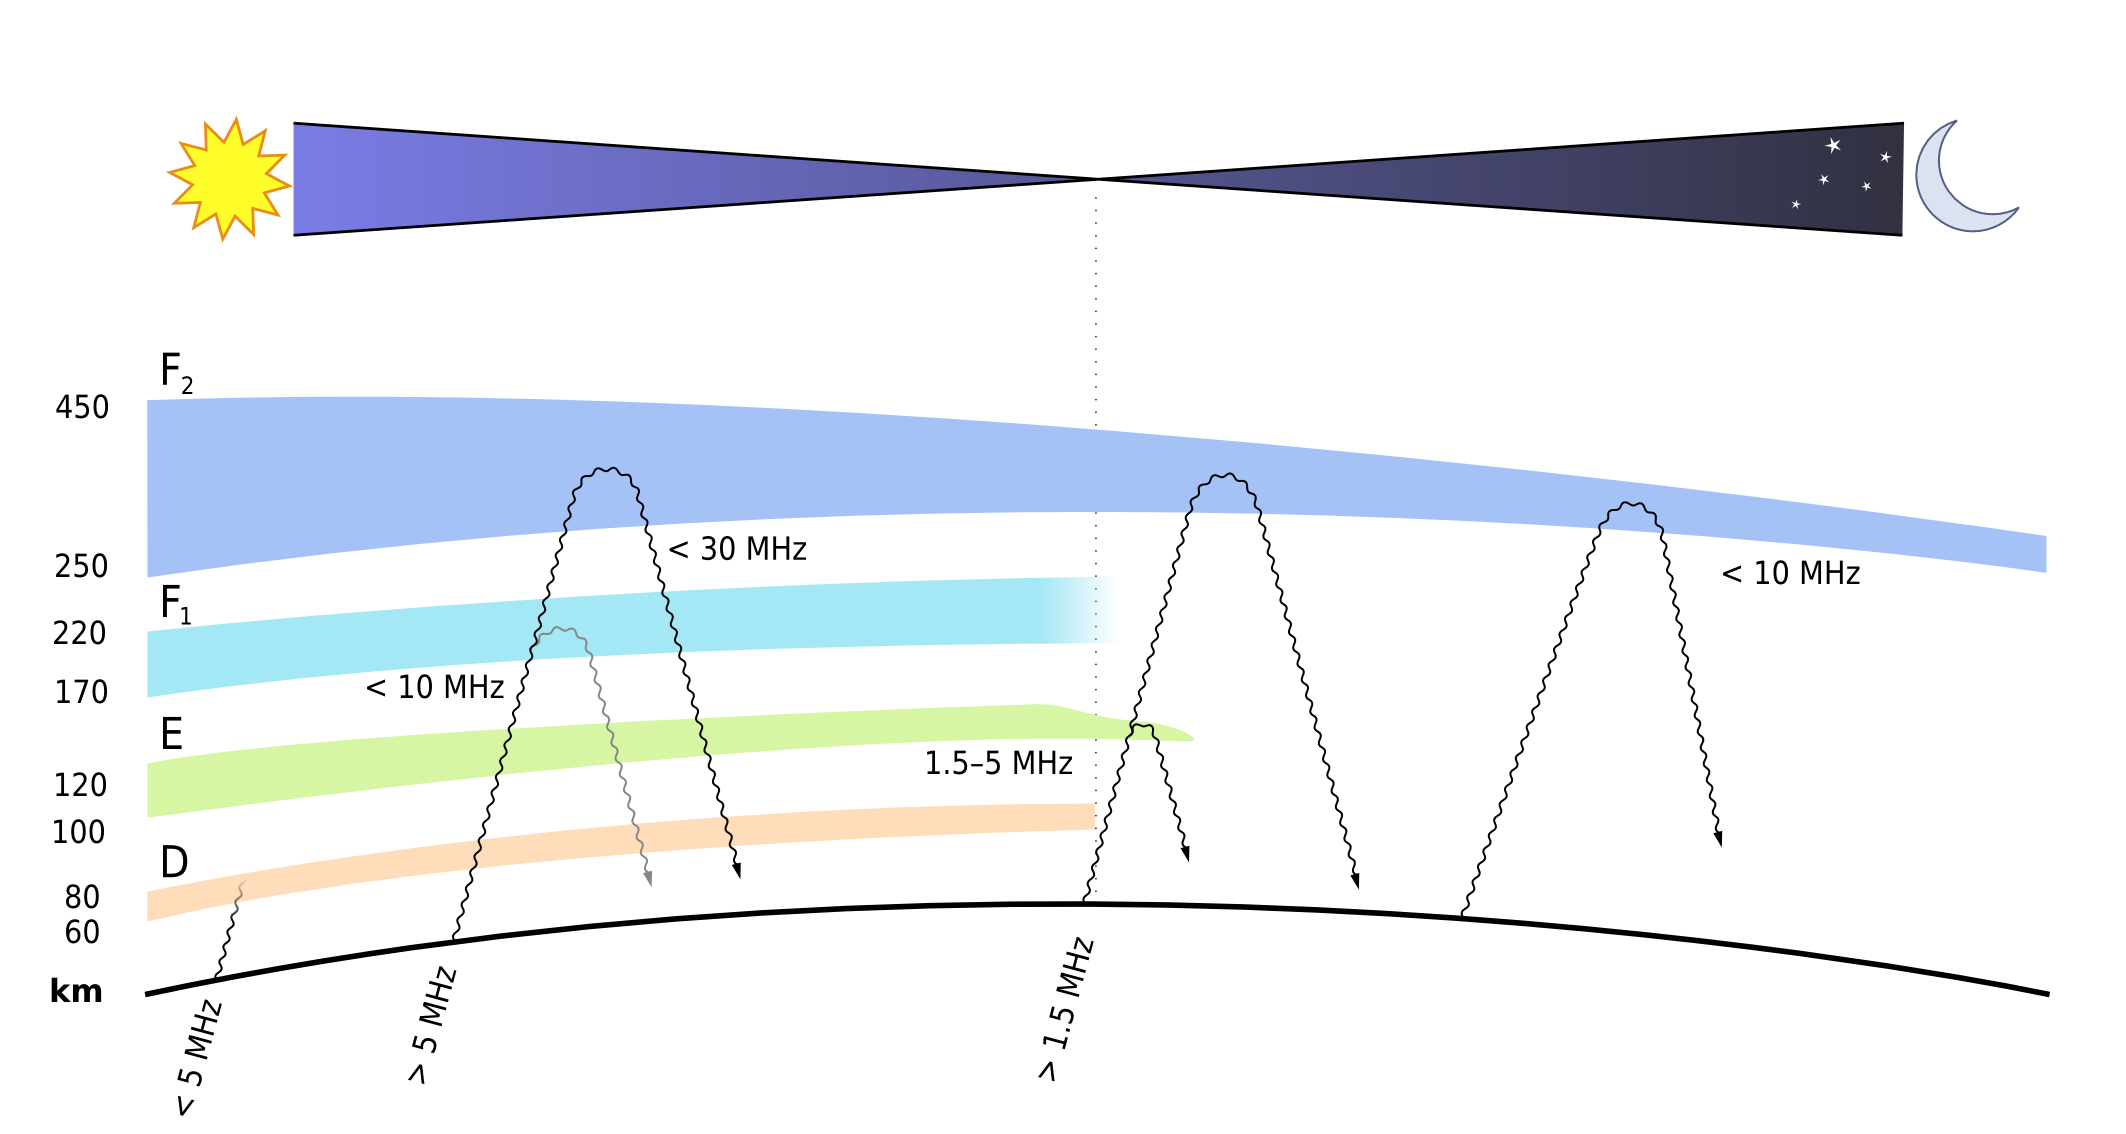
\includegraphics[width=11cm]{./png/Amfu-Ionosphere.png}
 \caption{Aufbau der Ionosphäre und reflektierende Eigenschaften der Schichten}
 \label{fig:ionosphere}
\end{figure}


Insgesamt besteht die Ionosphäre aus drei Schichten, die D-, E- und F-Schichten genannt werden. Die D-Schicht dämpft, die E-Schicht reflektiert tiefere Frequenzen und die F-Schicht höhere. Bei Sonneneinstrahlung (d. h. am Tag) werden Moleküle in der Ionosphäre durch Röntgen- und EUV\footnote{EUV: Extreme ultraviolette Strahlung mit Wellenlängen von 14 bis 80 nm}-Strahlung ionisiert. Eine weitere Rolle spielt die Sonnenfleckenzahl, die sich 2007 in einem Minimum befand und alle 11 Jahre ein Maximum erreicht. Je mehr Sonnenflecken vorhanden sind, desto stärker wird die Ionosphäre bei Sonneneinstrahlung ionisiert. Der Einfluss der Sonnenflecken ist nicht zu vernachlässigen; so sind HF-Frequenzen ab etwa 20 MHz während eines Minimums nicht verwendbar, in einem Maximum jedoch können weltweite Verbindungen beinahe den ganzen Tag entstehen.

\subsection{D-Schicht}
Die unterste der ionisierten Schichten existiert nur am Tag und reflektiert keine Signale. Tiefe Frequenzen unter 5 MHz werden so stark gedämpft, dass das 80-m- und das 160-m-Band nicht mehr benutzbar ist, auf höhere Frequenzen hat es keine grossen Auswirkungen.

Nach Sonnenuntergang verschwindet die D-Schicht sehr schnell, da die Ionen aufgrund der hohen Konzentration schnell wieder rekombinieren.

Bei sehr starker Sonnenaktivität kann der sogenannte \textit{Mögel-Dellinger-Effekt} auftreten. Dann ist die D-Schicht so stark ionisiert, dass das gesamte HF-Band für einige Minuten bis Stunden mehr oder weniger tot ist.

\subsection{E-Schicht}
Tagsüber dämpft die E-Schicht Frequenzen über 5 MHz, da die Ionenkonzentration für eine Reflexion zu gering ist. Tiefere Frequenzen werden reflektiert, müssen aber zuerst die D-Schicht passieren. Die Ionisierung befindet sich um die Mittagszeit in einem Maximum und verringert sich danach wieder langsam.

Nach Sonnenuntergang rekombiniert die E-Schicht innerhalb ungefähr einer Stunde nahezu vollständig. Innerhalb dieser Stunde kann sie für kurze Verbindungen über 500 km genutzt werden, da das 80-m- und 160-m-Band dann nicht mehr durch die D-Schicht gesperrt ist.

Im Sommer tritt manchmal manchmal die \textit{Sporadische E-Schicht} ($\textrm E_S$) auf. Es ist nicht klar, wie sie entsteht. An ihr wird sogar VHF reflektiert, was Überreichweiten und hohe Signalstärken ermöglicht. HF wird an einer tieferen Schicht als sonst reflektiert und erlaubt so Verbindungen über kürzere Distanzen von unter 500 km \textit{(Short Skip)}.

\subsection{F-Schicht}
Die F-Schicht ist die wichtigste für HF. Sie besteht am Tag aus zwei verschiedenen Schichten: Der $\mathrm F_1$- und der $\mathrm F_2$-Schicht. In der $\mathrm F_1$-Schicht werden neue Ionen gebildet, die stärkste Ionenkonzentration befindet sich in der $\mathrm F_2$-Schicht. 

Da sich in der Region der $\mathrm F_2$-Schicht nur noch wenige Gasmoleküle befinden, benötigen die Ionen sehr lange zur Rekombination. Sie besteht darum auch während der Nacht, die Stärke nimmt aber ab und somit auch die \link{MUF}.

\section{Arten der Wellenausbreitung}
\subsection{Bodenwelle} \label{sec:bodenwelle}
Die Bodenwelle \textit{(Ground Wave)} hat bei LF eine Reichweite von über 400 km\footnote{Bei gebirgigem Gelände etwa die Hälfte, bei Ozeanen u. ä. mehr als das Zweifache.}, bei HF reicht sie jedoch auf 80 m knapp 150, auf 10 m nur noch um die 30 Kilometer weit. Sie bewegt sich in der Troposphäre über dem Boden und wird hauptsächlich vom Boden gedämpft. Dabei wirken sich zum Beispiel dichte Vegetation (Wald), trockener Boden und stark bebaute Gebiete negativ auf die Reichweite aus, was aber zum Beispiel bei militärischen Einsätzen gewünscht sein kann. Gut leitende Untergrunde wie Wasser führen zu grösseren Reichweiten.

\subsection{Raumwelle}\label{sec:raumwelle}
Mit der Raumwelle \textit{(Sky Wave)}, die wie die Bodenwelle von jeder HF-Antenne erzeugt wird, ist es möglich, durch (Mehrfach-)Reflexionen an der Ionosphäre grössere Distanzen zu überbrücken. Pro Hop (Reflexion auf der Erde) können mehrere hundert Kilometer zurückgelegt werden, sogar bei Nacht noch über 500. Bei jeder Reflexion wird das Signal gedämpft.

Je flacher der Abstrahlwinkel der Antenne ist, desto höhere Frequenzen kann man verwenden und desto weiter kommt man mit einem Hop. Umgekehrt sollte für eine Nahverbindung eine tiefe Frequenz und ein steiler Abstrahlwinkel über 30° gewählt werden.

Für Verbindungen über weite Entfernungen eignen sich die Stunden um Sonnenauf- und -untergang am besten, da zu dieser Zeit die F-Schicht zwischen den Stationen gut aufgebaut ist. Beispiel: Bei Verbindungen in die USA gegen den Mittag wäre dort Nacht und die F-Schicht sehr dünn, so dass diese Frequenzen nicht reflektiert würden. Um Sonnenuntergang wird die F-Schicht hier langsam abgebaut, über dem Atlantik ist sie am stärksten, und in den USA wird sie gerade aufgebaut.

Die Raumwelle wird ab VHF zur Space Wave.

\subsection{Space Wave}
Die \textit{Space Wave} tritt ab VHF aufwärts auf. Sie bewegt sich quasi-optisch, also ungefähr bis zum Horizont, da sie kaum gebeugt wird und dann im All verloren geht. Allerdings wird sie zum Beispiel an Bergen reflektiert und von Wäldern und Häusern gedämpft, wodurch ihre Reichweite um einiges eingeschränkt wird. 

\section{QRN – Störungen in der Atmosphäre}
Vor allem unterhalb des 20-m-Bandes können atmosphärische Störungen eine solche Stärke erreichen, dass Gegenstationen trotz hoher Signalstärke nur noch schlecht hörbar sind. Im Sommer nimmt das QRN aufgrund häufigerer Blitzentladungen zu.

\subsection{Blitze}\label{sec:blitze}
Während der Entladung eines Blitzes entsteht ein elektromagnetischer Puls, da sich während einer kurzen Zeit extreme Spannungsänderungen vollziehen und gewaltige Ströme fliessen. Solche Störungen lassen sich in sehr weiter Distanz noch messen. Mit speziellen Systemen ist es sogar möglich, die Blitze zu orten. So können ungefähr 95\,\% der Blitze festgehalten werden.

Die von Blitzen erzeugten Signale werden \textit{Spherics}, \textit{Tweeks} oder \textit{Whistler} genannt, je nachdem, wie weit sie «gereist» sind. Spherics erzeugen im Wasserfalldiagramm nur Striche, Tweeks leicht gebogene Striche und Whistler hinterlassen Kurven, da Frequenzen höherer Wellenlänge schneller sind und so früher ankommen. Tweeks und Whistler sind als Pfeifton hörbar, dessen Frequenz sich ändert. Bei Tweeks dauert dies ein paar Hundertstelssekunden, Whistler wandern entlang des Erdmagnetfeldes und sind aufgrund der noch grösseren zurückgelegten Distanz länger hörbar – bis mehrere Sekunden lang. Sferics sind als kurzes Knacken hörbar.

\begin{figure}[h!]
 \centering
 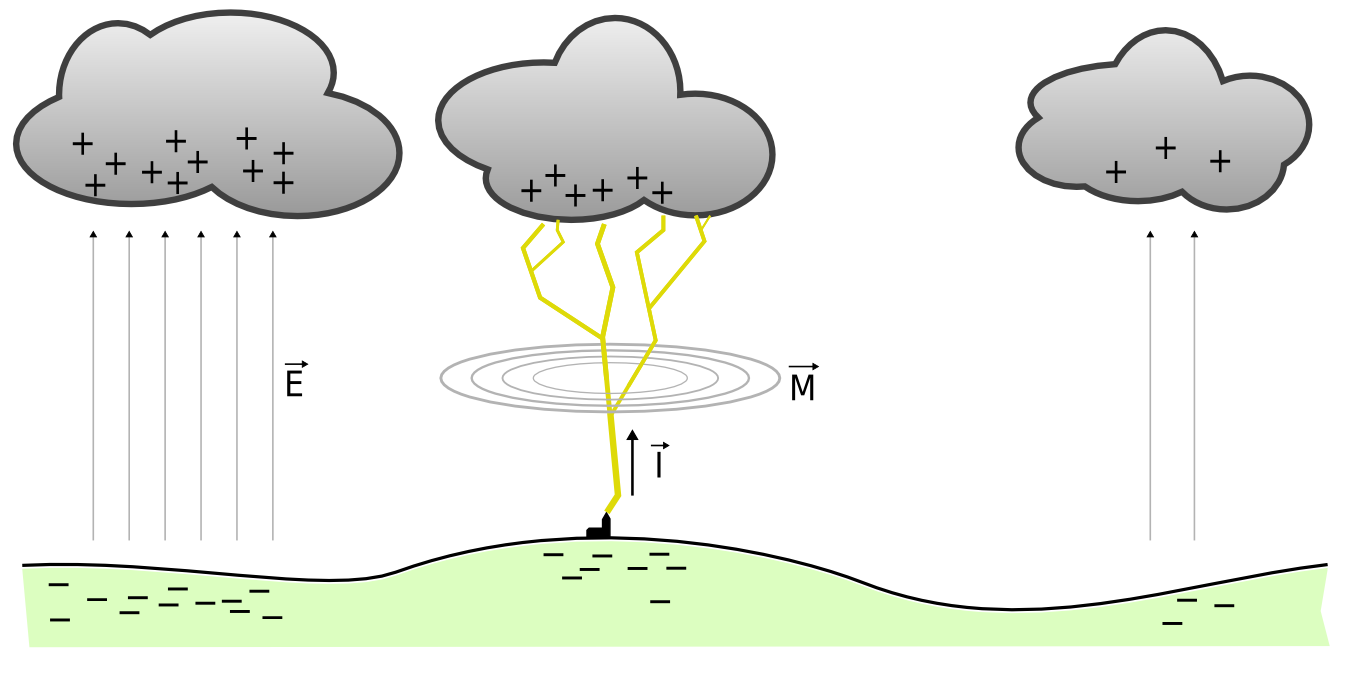
\includegraphics[width=11cm]{./png/Amfu-Blitz.png}
 \caption{Entladung eines Blitzes: Bei einem Gewitter besteht durch den Ladungsunterschied zwischen Wolke und Erde ein elektrisches Feld. Bei einem Blitz fliessen Elektronen (d. h. ein starker Strom) zur hier positiv geladenen Wolke, dadurch entsteht kurzfristig ein starkes magnetisches Feld.}
 \label{fig:blitz}
\end{figure}


Entladungen, die sich in der Nähe ereignen, erzeugen Störungen über das ganze Spektrum, hörbar in den unteren Bändern als starkes Knacken, in den oberen als kurz stark erhöhtes Rauschen.

\begin{figure}[h!]
 \centering
 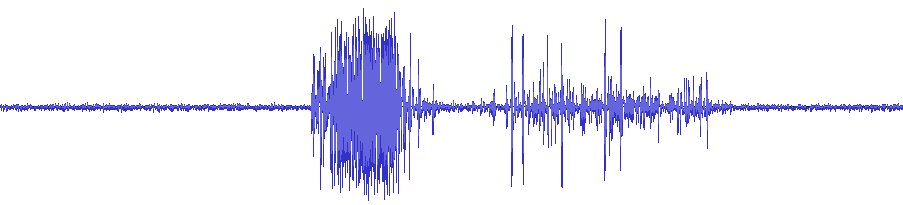
\includegraphics[width=5cm]{./png/Blitz-20M.png}
 \caption{Störung durch einen Blitz auf 21 MHz (Dauer des Ausschnittes: 2 Sekunden)}
 \label{fig:flash20}
\end{figure}


\section{QRM – Von Menschen verursachte Störungen}
QRM kann viele Ursachen haben. Auf Bändern mit hohem Funkverkehr können es ganz einfach andere Stationen sein, die so weit entfernt sind, dass sie nicht mehr verstanden, aber dennoch empfangen werden können und so den eigenen Funkverkehr stören. 

Eine andere häufige Störungsursache sind elektrische Geräte wie Computer, die in der Nähe laufen.





\end{document}
